\documentclass[bsc,frontabs,twoside,singlespacing,parskip,deptreport]{infthesis}

\usepackage[round]{natbib}
\usepackage[hidelinks]{hyperref}

\usepackage{graphicx}

% For nice references including the words Figure, Section, etc
\renewcommand*{\sectionautorefname}{Section}%
\renewcommand*{\subsectionautorefname}{Section}%
\renewcommand*{\figureautorefname}{Fig.}%
\newcommand{\algorithmautorefname}{Alg.}

\begin{document}

\title{\vspace{-5.0cm} \centering{\includeshield} \vspace{1cm} \\ Prosodic features in state-of-the-art \\spoken language identification}

\author{Sam Sucik}

\course{Master of Informatics}
\project{\vspace{3cm}{\bf MInf Project (Part 1) Report}}

\date{2019}

\abstract{
  TO-DO
}

\maketitle

% Add acknowledgements if necessary.
\section*{Acknowledgements}{
  Thanks to Paul Moore for productive collaboration while building the baseline system, to Steve Renals for his supervision and optimism, and to David Snyder for his advice.
}

\tableofcontents

\chapter{Introduction}{
  \section{Motivation}{
    LID is useful in ASR, in voice assistants, emergency call routing, etc.
    Traditionally, acoustic features are used (influence of ASR on LID and SID). Prosodic LID is much rarer, although results show that prosodic information can help identify language \citep{Lin_et_al_2005}, and that both LID and ASR can benefit from using acoustic \textit{and} prosodic features \citep{Martinez_et_al_2013,Ghahremani_et_al_2014}.
    Just last year, a novel architecture for LID utilising \textit{x-vectors} was proposed by \cite{Snyder_et_al_2018}, dramatically improving the state-of-the-art results. Although the authors find that using bottleneck features from an ASR DNN yields better results than using the standard acoustic MFCC features, even the ASR DNN was trained just using MFCCs. Thus the work ignores the potential of speech information other than that captured by MFCCs.
  }
  \section{Aims}{
    In this work, I aim to reproduce the state-of-the-art x-vector LID system and explore the use of prosodic features in addition to acoustic ones. Because the system uses a relatively novel architecture, in which a TDNN aggregates information across a speech segment, I also compare two types of acoustic features, one which has such aggregation over time encoded (SDC) and one that only containes information about single frames (vanilla MFCC).
  }
  \section{Contributions}{
    \begin{enumerate}
      \item {
        Adapted an existing x-vector speaker verification implementation (based on \cite{Snyder_et_al_2018b}) for language identification
      }
      \item {
        Explored the choice of classifiers and chose a different one than \cite{Snyder_et_al_2018}
      }
      \item {
        Prepared the Global Phone corpus for LID with the x-vector system, extending the original partitioning of the corpus into datasets and analysing invalid data
      }
      \item {
        Built and evaluated a baseline, end-to-end x-vector LID system using 19 languages of the Global Phone corpus
      }
      \item {
        Explored, set and tuned important hyperparameters of the system, mainly the number of training epochs of the x-vector TDNN
      }
      \item {
        Researched literature concerning the use of acoustic and prosodic features in language identification, speaker verification and ASR
      }
      \item {
        Designed, run and evaluated experiments comparing two types of acoustic features (MFCC and SDC) and two prosodic features (pitch, energy), and their combinations
      }
      \item {
        Built a system which has the potential to be open-sourced as part of the Kaldi ASR toolkit, to be used by a wider community
      }
    \end{enumerate}
  }
}

\chapter{Background}{
  \label{chap:Background}
  This chapter elaborates on the key concepts relevant to my work, as shown in this condensed description of the project: Exploring \textbf{spoken language identification} in the context of the recently proposed \textbf{x-vector} system (contrasted with the more established state-of-the-art \textbf{i-vector} approach), focusing on utilising \textbf{prosodic information} in addition to the standard \textbf{acoustic information}.

  \section{The task: spoken language recognition}{
    \label{sec:LID}
    Spoken language recognition means recognising the language of a speech segment. The task is similar to speaker recognition and, in the past, similar systems have been used for the two tasks. Importantly, recognition is typically realised as one of two different tasks: 
    \begin{itemize}
      \item {Identification (multi-class classification): answering the question "For a speech segment $X$, which one (from a number of supported targets) is its target (language or speaker) $T_x$?"}
      \item {Verification (binary classification): "Is $T_x$ the target (language or speaker) of the speech segment $X$?"}
    \end{itemize}
    Identification is more suitable for use cases with a small and stable set of possible targets -- such as the set of supported languages. There, computing the probability of $T_x$ being each of the target languages is feasible. Verification, on the other hand, is more suitable for cases where the set of possible targets less constrained -- such as the large and changing set of possible speakers in speaker verification systems. There, it is often infeasible to compute the probability distribution over all possible values of $T_x$; instead, the system typically focuses only on evaluating the probability of $T_x$ being the hypothesised speaker. Throughout this work, I focus on \textit{language identificaion} (LID) with a \textit{closed set} of target languages (i.e. not including the option to identify a speech segment's language  as unknown/other).
  }

  \section{Shallow utterance-level approach to LID: i-vectors}{
    \label{sec:i-vectors}
    This approach, with its numerous variations, has now been the state of the art for 8 years -- since first introduced by \cite{Dehak_et_al_2011} for speaker recognition and later applied by \cite{Martinez_et_al_2011} in language recognition.
    
    \begin{figure}[h!]
      \centering
      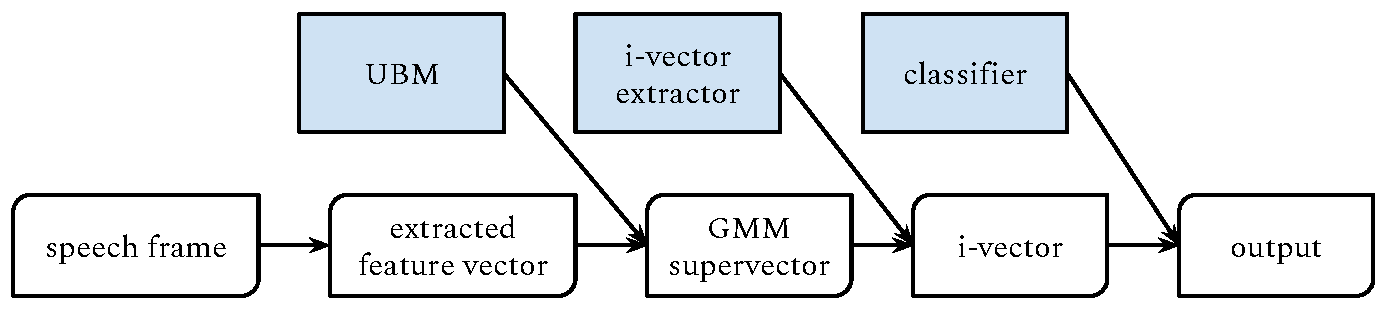
\includegraphics[width=14.5cm]{graphics/i-vectors}
      \vspace*{-1em}
      \caption{Language identification using a typical i-vector system.}
      \label{fig:i-vector}
    \end{figure}

    The main components of a typical i-vector system, together with their use for prediction, are shown in \autoref{fig:i-vector}. The universal background model (UBM) is a Gaussian mixture model (GMM) consisting of a large number (e.g. 2048) multivariate mixture components. The UBM is trained using the Expectation-Maximisation algorithm to model the observation space of frame-level feature vectors $\mathbf{x}$ computed from all training utterances (typically 39-dimensional vector using the MFCC features, see \autoref{sec:acoustic-feats}). Given the trained UBM, an utterance $X$ can be represented by a language- and channel-specific GMM supervector $M$ as:
    \begin{equation}
      \label{eq:supervector}
      M_X = m + Tw_X
    \end{equation}
    Here, $m$ is the language- and channel-independent GMM supervector of the UBM (consisting of the stacked means of all mixture components). $T$ is the \textit{total variability matrix} -- also called the i-vector extractor, and $w_x$ is the \textit{identity vector} (i-vector) of sample $X$. The total variability matrix $T$ is "a matrix of bases spanning the subspace covering the important [language and channel] variability in the supervector space" (\citeauthor[p.862]{Martinez_et_al_2011}). Effectively, $T$ projects between the high-dimensional GMM supervector space and the low-dimensional \textit{total variability subspace} (also called the \textit{i-vector space}). The i-vector $w_x$ is then a low-dimensional set of factors projecting the supervector onto the total variability subspace base vectors. The i-vector extractor $T$ is trained again using Expectation-Maximisation (for details see \citet[p. 100]{ivector_tutorial}). Without providing too much detail, I highlight the aspect that is most relevant to my work: training $T$ is based on calculating and further combining the 0\textsuperscript{th}, 1\textsuperscript{st} and 2\textsuperscript{nd} order statistics which are computed by \textit{summing over the frames} of an utterance.

    Once the i-vector extractor has been trained, any utterance can be represented by its i-vector. This enables training a relatively simple and fast classifier operating over the low-dimensional i-vectors. Different classifiers have been successfully used with the i-vector back end; for example, \citeauthor{Martinez_et_al_2011} initially tried using these, all achieving roughly equal performance:
    \begin{enumerate}
      \item {a linear generative model -- modelling the i-vectors of each language by a Gaussian, with a shared full covariance matrix across all language-modelling Gaussians}
      \item {a linear Support Vector Machine computing scores for all languages by doing binary classification in the one-versus-all fashion}
      \item {a two-class logistic regression also doing one-versus-all classification.}
    \end{enumerate}

    At test time, a sequence of feature vectors for utterance $X$ is projected using the UBM into the high-dimensional \textit{supervector space}, producing $M_X$. Then, $T$ is used to extract the utterance-level i-vector, which is processed by the classifier.

    Despite producing utterance-level scores, I describe the i-vector pipeline as shallow because it aggregates frame-level information over time very early (when projecting $X$ into the supervector space), effectively treating an utterance as a bag of frames and disregarding any temporal patterns spanning over multiple frames.
  }

  \section{Less shallow approach: d-vectors}{
    \label{sec:d-vectors}
    % in short: creating utterance-level representations by extracting frame-level information and averaging over frames
    % main difference compared to i-vectors: looking at sequences, i.e. taking each frame's surrounding context into account (this was done by both Variani and Tkachenko)
    % context aggregation done using standard DNN but Tkachenko used TDNN, more familiar from ASR acoustic models
    % describing TDNN: like 1D CNN, but often made sparse. aggregates information along the time axis
    Introduced for speaker verification by \citet{Variani_et_al_2014} and later adapted and applied to language identification by \citet{dvectors_lid}, this approach uses deep neural networks to extract frame-level information, which is then averaged across frames to produce utterance- or language-level representations.
  }

  \section{Deep utterance-level approach: x-vectors}{
    \label{sec:x-vectors}
    As opposed to the frame-level i-vector systems, this approach, introduced last year by the John Hopkins University team first for speaker verification \citep{Snyder_et_al_2018b} and subsequently for language identification \citep{Snyder_et_al_2018}, aggregates information over time and produces scores at segment level, even for variable-length speech segments. It is attractive also because \citeauthor{Snyder_et_al_2018} report beating the i-vector state-of-the-art system on the LID task.

    TO-DO: add a diagram of the pipeline, define TDNN and x-vectors properly
    
    In 2018, the Johns Hopkins University team -- \cite{Snyder_et_al_2018} -- introduced a system which uses deep convolutional neural networks (referred to as time-delay neural networks -- TDNN) to aggregate and process information across the frames of a variable-length speech segment. Such TDNN is trained to do direct language classification. Empirically, however, better results are achieved when low-dimensional embeddings called \textit{x-vectors}, representing entire segments, are extracted from the trained TDNN and scored by a separate trained classifier. This system is attractive not just because of the promising performance: It no longer operates on the frame level; instead, it has the potential to effectively aggregate low-level information over multiple frames and do further processing. As demonstrated by the authors, when using a separate classifier, the architecture also supports -- without much impact on the LID performance -- extending the set of target languages without having to expensively re-train the x-vector TDNN. It is enough to train the light-weight classifier.
  }
  \section{Features used in language identification}{
    TO-DO: Add more references.

    Mention that acoustic are more accent-independent while prosodic may be misleading e.g. for non-native speakers.

    Historically, ASR has been the main point of focus among all speech processing areas, which is reflected in today's dominant use of acoustic features -- primarily developed for ASR -- in other tasks like LID and SID. These acoustic features, the most popular ones being MFCC, Mel filterbank and SDC, are not necessarilly best-suited for the other tasks. For instance, all three disregard any pitch information -- which makes sense in the context of ASR, where intonation is typically ignored, but is certainly not desirable in speaker identification, where intonation and the pitch range contribute to speaker-specific characteristics. Another ASR-inspired approach to LID is the \textit{phonotactic} one, which exploits the different phone distributions across languages.

    In this work, I acknowledge \textit{acoustic} LID (using acoustic features), but \textit{prosodic} LID receives the most attention -- using features which are disregarded in ASR, but have a great potential in language and speaker identification tasks.

    \subsection{Acoustic features}{
      \label{sec:acoustic-feats}
      Definitions of MFCCs and SDCs, probably ignore PLPs, Mel filterbanks, etc

      SDC used by \cite{Ferrer_et_al_2016} and \cite{Sarma_et_al_2018} (7D MFCC + 7-1-3-7 SDCs = 56D) and by \cite{Torres-Carrasquillo_et_al_2002} (10-1-3-3)

      19 MFCCs + energy + 20 $\Delta$ + 20 $\Delta\Delta$ = 60D by \cite{Sarma_et_al_2018} -- outperformed by SDCs, but note that they trained an ASR TDNN for generating i-vectors
      
      MFCCs also used inderectly to train ASR DNNs which then provide bottle-neck features which give very promising results in both LID and SID
    }
    \subsection{Prosodic features}{
      Elaborate on prosody as consisting of intonation (F0), stress (energy) and rhythm (segment durations).
      
      39D MFCC vectors combined with 4D pitch features \citep{Song_et_al_2013}

      \cite{Lin_et_al_2005} do LID just from the pitch contour parametrised by Legendre polynomials

      \cite{Ghahremani_et_al_2014} show ASR improvements with a pitch-tracking algorithm that calculates pitch even for unvoiced frames
    }
  }
}

\chapter{Data}{
  Intro: Historically, speech corpora were meant for ASR, but now used for LID and SID as well. Since 1996, NIST has also been organising Language Recognition Challenges (LREs), and the corpora used for LREs are now the typically used ones when it comes to evaluating different systems. However, NIST traditionally focuses on telephone, narrowband (8kHz) speech, which represents only one part of all the possible settings in which LID or SID are deployed. In this work, I use a relatively small (< 40GB) corpus which, however, has many qualities that the various NIST corpora lack.

  \section{GlobalPhone}{
    Presented by \cite{Schultz_et_al_2013}, originally for ASR. Wideband (16kHz), recorded native speakers of 23 languages reading newspaper articles -- very similar to the English corpora such as CSR-I, which are based on Wall Street Journal articles. Unlike in NIST corpora, the recording equipment and conditions vary very little. One disadvantage of GlobalPhone is the lack of spontaneous speech. On the other hand, the language goes well beyond the simple conversational language found in the NIST telephone speech corpora.
  }

  \section{Data partitioning}{
    GlobalPhone comes with a partitioning of each language's data into training, development and evaluation datasets, with the sizes of the datasets being roughly 80\%, 10\%, 10\%, respectively. However, for the purposes of the x-vector architecture, 4-way partitioning is required:
    \begin{enumerate}
      \item{training set -- for training the x-vector TDNN,}
      \item{enrollment set -- for training the x-vector classifier,}
      \item{evaluation set ('development' in the GlobalPhone terminology) -- for tuning the hyperparameters of both the TDNN and the classifier,}
      \item{testing set -- for final performance evaluation on unseen data.}
    \end{enumerate}

    In order to use GlobalPhone with the x-vector system, I allocated part of the training data for enrollment. I tried to preserve the GlobalPhone development sets and evaluation sets (which I refer to as evaluation and testing sets, respectively), in order to enable fair comparison of my results obtained on those data portions with any other works that use the GlobalPhone corpus.

    Taking into account the relatively small number of parameters of the x-vector classifier when compared to the x-vector TDNN, I split the training data such that approximately only one 8th is used for enrollment. This way, the training data accounts for roughly 70\% of the whole corpus, while the 3 other portions are roughly 10\% each.

    Importantly, GlobalPhone (as of the GlobalPhone Documentation v4.1) still misses the partitioning for certain languages:
    \begin{enumerate}
      \item {no partitioning for Czech, Polish, Tamil, Swahili, Ukrainian, Vietnamese and Shanghai Chinese,}
      \item {only partial partitioning for Arabic, French, Japanese, Russian.}
    \end{enumerate}

    The {\texttt GlobalPhone} Kaldi recipe contains an extended partitioning, which fixes Czech, French, Japanese, Polish, Russian, Swahili and Vietnamese. For the rest of the languages with incomplete partitioning (Arabic, Tamil, Ukrainian and Shanghai Chinese), I created the partitioning myself, following the same approach as the GlobalPhone authors: "No speaker appears in more than one group and no article was read by two speakers from different groups" (TO-DO: reference the GP docs).

    Some languages didn't have speaker-article data; for those, the partitioning was done randomly.

    For some languages, I could not construct a partitioning with zero article overlap; for those, I tried to at least minimise the overlap.    
  }

  \section{Initial data preprocessing}{
    Basically, SHN to WAV

    Splitting long utterances into shorter ones uniformly, to be able to do classifier training and end-to-end evaluation on segments of different lengths -- like in \cite{Snyder_et_al_2018}. One future improvement would be to not do uniform splitting, but rather split on breaks -- to prevent potentially bad edge effects.
  }

  \section{Invalid data}{
    This was discovered while preprocessing the data from .shn to .wav:
    \begin{enumerate}
      \item {Hausa, Swahili and Ukrainian have broken data.}
      \item {Bulgarian, German, Russian, Turkish and Vietnamese have one broken utterance recording each -- not a big deal, as the number of utterances per language is in hundreds.}
      \item {Portuguese has 2 speakers with almost all data broken (these were discarded), and other 10 speakers with up to 3 broken utterance recordings each (these were keps)}
    \end{enumerate}

    This leaves us with 19 languages, which are used further in this work: Arabic (AR), Bulgarian (BG), Mandarin Chinese (CH), Croatian (CR), Czech (CZ), French (FR), German (GE), Japanese (JA), Korean (KO), Polish (PL), Portuguese (PO), Russian (RU), Spanish (SP), Swedish (SW), Tamil (TA), Thai (TH), Turkish (TU), Vietnamese (VN) and Shanghai Chinese (WU).
  }
}

\chapter{Implementation}{
  \section{The Kaldi toolkit}{
    System was built in Kaldi \citep{Povey_et_al_2011}. (Introduce Kaldi.)
  }
  \section{Adapted implementations}{
    Describe the SRE16 Kaldi recipe, the GlobalPhone ASR recipe, and how they were combined (also using the information from \cite{Snyder_et_al_2018}) to reproduce the LID x-vector system.
  }

  \section{Choice of classifier}{
    The SRE16 recipe uses PLDA, but for verification, not for classification. For our purposes, we needed a proper classifier. Current popular and well-performing classifiers are various flavours of GMM and logistic regression, with no clear winner. \cite{Snyder_et_al_2018}, for instance, used GMM trained using MMI -- based on \cite{McCree_2014}. I decided to re-use a model which is already implemented in the LRE07/v2 Kaldi recipe -- logistic regression. The decision was also consulted with \cite{Snyder_2018_kaldi-help}. One theoretical downside of logistic regression is that the resulting decision boundaries are linear, whereas with GMM (trained with full co-variance matrix), one can achieve more complex quadratic decision boundaries. On the other hand though, training a full covariance requires much data, and the enrollment set would likely be not big enough. Additionally, the Kaldi logit can describe each class using more than linear boundary (see next section), so the decision boundaries should be complex enough to be able to model the observed data well.
  }

  \section{Final architecture}{
    Description of x-vector+GP architecture (highlighting own contributions)

    how the whole pipeline works: go into much more detail than in the Related work section

    description of the Kaldi logit, which models each class using multiple "mixtures", i.e. multiple boundaries
    
    mention possibility of direct classification with TDNN and that I focus on using separate classifier because it provides extra flexibility and because it was shown to perform slightly better
  }

  \section{Computing environment}{
    cluster, Slurm, GPUs, parallelisation, rough runtimes of the different stages (TDNN training, x-vector extraction, logit training, inference)
  }

  \section{Hyperparameters}{
    decided: TDNN layers, activation function, learning algorithm (TO-DO: read about shrinking)

    tuned (using the baseline setting, see next chapter): number of TDNN training epochs, logit hyperparameters
  }
}

\chapter{Experiments}{
  Intro: I will compare a selection of acoustic and prosodic features. Despite their reported potential, I don't use BNFs in this work, as they are basically just a higher-level feature based on the acoustic MFCC information (at least the BNFs in \cite{Snyder_et_al_2018}).

  Evaluation metric: $C_{primary}$, consistent with NIST LREs. Elaborate a bit more on the meaning of the metric, maybe compare with accuracy and other simpler metrics.

  \section{Baseline}{
    vanilla MFCCs (no deltas): also comment on the decisions made regarding MFCC MFCC configuration

    $\leq 30s$ enrollment segments, $\leq 10s$ eval/test segments (should be possible to also report exact average segment length for each set)
  }

  \section{Shifted delta cepstra}{
    Want to see whether context aggregation in the form of added deltas in SDCs (compared to vanilla MFCCs) can improve performance, since the TDNN does context aggregation of its own.
  }

  \section{KaldiPitch+Energy vectors}{
    Calculating pitch even for unvoiced frames using the algorithm presented by \cite{Ghahremani_et_al_2014}. Adding raw energy to model stress. Extremely low-dimensionality feature vectors, but will see how the TDNN and classifier trained on these can do prosodic LID. Hoping to achieve some sensible results, probably much worse than with MFCCs or SDCs.
  }
  
  \section{MFCC/SDC + KaldiPitch+Energy}{
    Taking the winner from MFCC/SDC, and concatenating those features with Kaldi pitch and raw energy values. Training the TDNN and classifier on that. Hopefully, seeing an improvement.
  }
  
  \section{Fusion of MFCC/SDC and KaldiPitch+Energy scores}{
    Stretch goal, likely to be delayed for Year 5 (or abandoned if there are more attractive ideas)

    Same as previous section, but scores computed separately (using two systems, one trained on acoustic features, the other one on prosodic) and fused using a logit fuser. Probably using evaluation set for training the fuser (although, ideally, a separate data portion would be reserved for that).
  }

  \section{Timeline for the experiments}{
    \label{timeline}
    \begin{enumerate}
      \item {
        Finished: System using MFCC and SDC.
      }
      \item {
        By January 28th: Choose the TDNN and logit hyperparameters. TDNN using MFCCs has already been trained for, 2, 3, ... 10 epochs, now need to 1) establish reasonable logit parameters (driven by evaluation-set performance on x-vectors from TDNN trained for 3 epochs), 2) use that logit config to score the TDNNs with different number of training epochs, 3) choose a number of epochs that is a reasonable compromise between performance and training runtime
      }
      \item {
        By February 4th: Have MFCC vs SDC comparison carried out (includes baseline results using MFCCs). Have KaldiPitch and raw energy features implemented (both are straightforward to compute with Kaldi -- the energy is just computing MFCCs with raw log energy instead of C0, and discarding all but the energy-corresponding resulting coefficient). Have splicing of MFCC/SDC features with prosodic features implemented.
      }
      \item {
        By February 11th: Have results of KaldiPitch+Energy experiments and of the acoustic+prosodic experiment (MFCC/SDC + KaldiPitch+Energy)
      }
    \end{enumerate}
  }
}

\chapter{Results}{
  Reporting: overall $C_{primary}$, accuracy (for illustrative purposes), confusion matrix (to see which language pairs are confusing)
  
  Focus on Slavic languages, since there is so many of them (Czech, Croatian, Polish, Russian, Bulgarian) and intonation can be very characteristic and important here (my own intuition, based on my knowledge of Slavic languages).
}

\chapter{Discussion}{
  
}

\chapter{Future work}{
  \section{Plans for Part 2 of the MInf project}{

  }

  \section{Other future ideas}{
    Everything that is sensible but unlikely in Year 5.
  }
}

\chapter{Conclusions}{
  
}

% use the following and \cite{} as above if you use BibTeX
% otherwise generate bibtem entries
\bibliographystyle{apalike}
\bibliography{s1513472-minf1}

\end{document}
